% begin module area-between-curves-def
\begin{frame}[t]
\begin{tabular}{|c|c|}
\hline
 \ \ \ \ \ The Area Under a Curve \ \ \ \ \ &
 \ \ \ \ The Area Between Two Curves \ \ \ \ \\
\psset{xunit=1.4cm, yunit=1.4cm}
\begin{pspicture}(-0.5, -0.5)(1.5,1.5) 
\psframe*[linecolor=white](-0.5,-0.5)(1.5,1.5) 
\tiny 
\psaxes[ticks=none, labels=none]{<->}(0,0)(-0.2,-0.3)(1.5,1.5)
\psLabels{1.5}{1.5}
\psXTickWithLabel{0.2}{$a$}
\psXTickWithLabel{1.1}{$b$}
\only<1>{ %
\pscustom*[linecolor=\psColorAreaUnderGraph]{%
\psplot[plotpoints=1000]{0.2}{1.1}{x -1 add 2 exp -1 mul 1.2 add }
\psline(1.1, 0)(0.2,0)
} %
} %
\rput[l](1,1.3){$y=f(x)$}
\only<handout:0| 2->{ %
\pscustom*[linecolor=\psColorAreaUnderGraph]{ %
\psline(0.35,0)(0.35,0.95)(0.65,0.95)(0.65,0)
} %
\psline{<->}(0.35,0.5)(0.65,0.5)
\rput[t](0.5,0.45){$\Delta x$}
\rput[b](0.5,1.1){$(x, f(x))$}
\psFullDot{0.5}{0.95}
} %
%Function formula: 6/5- ((-1+x)^{2}) 
\psplot[linecolor=\psColorGraph, plotpoints=1000]{0}{1.5}{x -1 add 2 exp -1 mul 1.2 add }
\end{pspicture} 
%\ \only<1>{%
%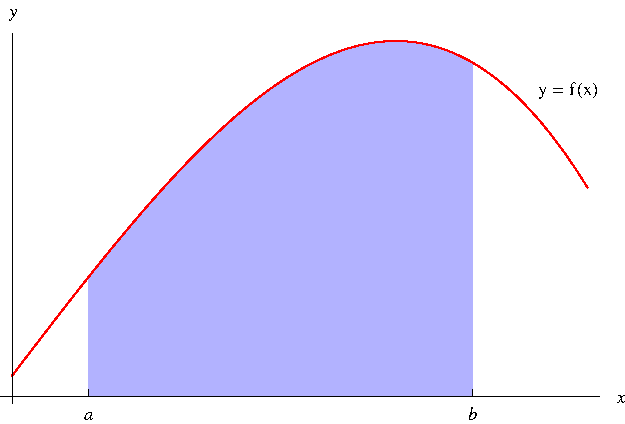
\includegraphics[height=3cm]{area-between-curves/pictures/06-01-singleint.pdf}%
%}%
%\only<handout:0| 2->{%
%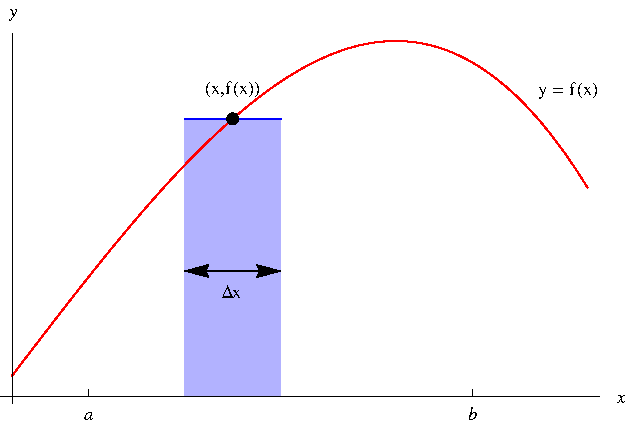
\includegraphics[height=3cm]{area-between-curves/pictures/06-01-1rectangle.pdf}%
%}
&%
\psset{xunit=0.65cm, yunit=0.65cm}
\begin{pspicture}(-0.5, -5)(4,5) 
\psframe*[linecolor=white](-0.5,-5)(4,5) 
\tiny 
\psaxes[ticks=none, labels=none]{<->}(0,0)(-0.5,-0.5)(4,3.5)
\psLabels{4}{3.5}
\psXTickWithLabel{0.5}{$a$} 
\psXTickWithLabel{3}{$b$}
\rput[bl](3.1, 3){$y=f(x)$}
\rput[l](3.1, 1.3){$y=g(x)$}
\only<-12>{ %
\pscustom*[linecolor=\psColorAreaUnderGraph]{ %
%Function formula: (1/4 (x))^{2}+2 
\psplot[plotpoints=1000]{0.5}{3}{2 x 0.25 mul 2 exp add } 
%Function formula: 3/2- ((-3/4+1/4 (x))^{2}) 
\psplot[plotpoints=1000]{3}{0.5}{x 0.25 mul -0.75 add 2 exp -1 mul 1.5 add }
} %
} %
\only<handout:0| 13->{ %
\pscustom*[linecolor=\psColorAreaUnderGraph]{ %
\psline(1.6, 1.4375)(1.6,2.25)(2.4, 2.25)(2.4,1.4375)
} %
\psFullDot{2}{2.25}
\psFullDot{2}{1.4375}
\psline{<->}(1.6,1.85)(2.4,1.85)
\rput[t](2,1.8){$\Delta x$}
\rput[t](2,1.2){$(x, g(x))$}
\rput[b](2,2.5){$(x, f(x))$}
} %
%Function formula: (1/4 (x))^{2}+2 
\psplot[linecolor=\psColorGraph, plotpoints=1000]{0}{4}{2 x 0.25 mul 2 exp add } 
%Function formula: 3/2- ((-3/4+1/4 (x))^{2}) 
\psplot[linecolor=\psColorGraph, plotpoints=1000]{0}{4}{x 0.25 mul -0.75 add 2 exp -1 mul 1.5 add }
\end{pspicture} 
%\ \only<-12>{%
%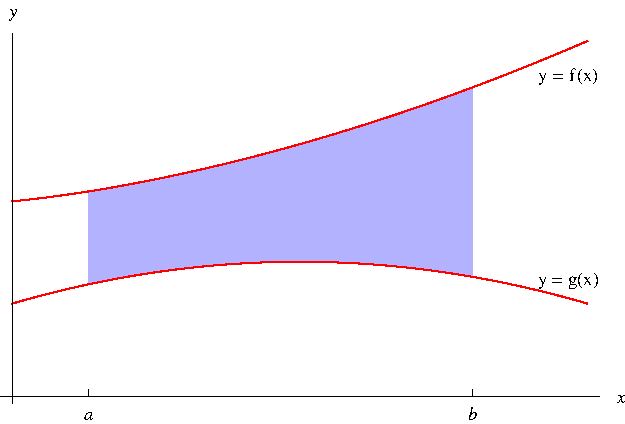
\includegraphics[height=3cm]{area-between-curves/pictures/06-01-doubleint.pdf}%
%}%
%\only<handout:0| 13->{%
%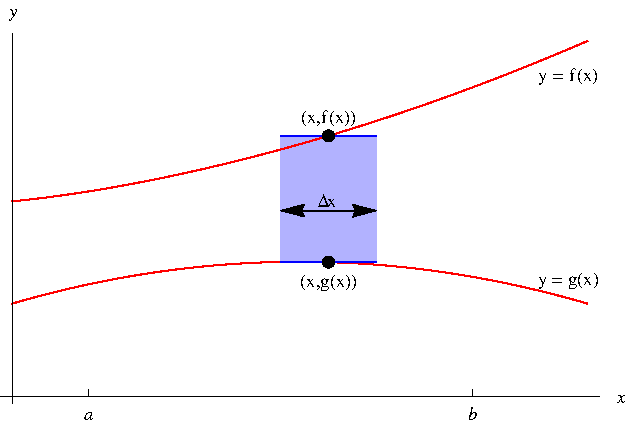
\includegraphics[height=3cm]{area-between-curves/pictures/06-01-1rectanglediff.pdf}%
%}
\\%
\uncover<2->{
rectangle area $ = $ \only<handout:0| -5>{\alert<handout:0| 5>{height}}\only<6->{\alert<handout:0| 6>{$f(x)$}}$\cdot$\only<handout:0| -3>{\alert<handout:0| 3>{width}}\only<4->{\alert<handout:0| 4>{$\Delta x$}}
} &
\uncover<13->{
rectangle area $ = $ \only<handout:0| -16>{\alert<handout:0| 16>{height}}\only<17->{\alert<handout:0| 17>{$(f(x)-g(x))$}}$\cdot$\only<handout:0| -14>{\alert<handout:0| 14>{width}}\only<15->{\alert<handout:0| 15>{$\Delta x$}}
} \\
\uncover<7->{%
\psset{xunit=1.4cm, yunit=1.4cm}
\begin{pspicture}(-0.5, -0.5)(1.5,1.5) 
\psframe*[linecolor=white](-0.5,-0.5)(1.5,1.5) 
\tiny 
\psaxes[ticks=none, labels=none]{<->}(0,0)(-0.2,-0.3)(1.5,1.5)
\psLabels{1.5}{1.5}
\psXTickWithLabel{0.2}{$a$}
\psXTickWithLabel{1.1}{$b$}

\only<7>{
\psline*[linecolor=\psColorAreaUnderGraph, linewidth=0.1pt](0.2, 0)(0.2, 0.56)(0.425, 0.56)(0.425, 0)(0.425, 0)(0.425, 0.869375)(0.65, 0.869375)(0.65, 0)(0.65, 0)(0.65, 1.0775)(0.875, 1.0775)(0.875, 0)(0.875, 0)(0.875, 1.18437)(1.1, 1.18437)(1.1, 0)
\psline[linecolor=blue, linewidth=0.1pt](0.2, 0)(0.2, 0.56)(0.425, 0.56)(0.425, 0)(0.425, 0)(0.425, 0.869375)(0.65, 0.869375)(0.65, 0)(0.65, 0)(0.65, 1.0775)(0.875, 1.0775)(0.875, 0)(0.875, 0)(0.875, 1.18437)(1.1, 1.18437)(1.1, 0)
}
\only<8>{
\psline*[linecolor=\psColorAreaUnderGraph, linewidth=0.1pt](0.2, 0)(0.2, 0.56)(0.3125, 0.56)(0.3125, 0)(0.3125, 0)(0.3125, 0.727344)(0.425, 0.727344)(0.425, 0)(0.425, 0)(0.425, 0.869375)(0.5375, 0.869375)(0.5375, 0)(0.5375, 0)(0.5375, 0.986094)(0.65, 0.986094)(0.65, 0)(0.65, 0)(0.65, 1.0775)(0.7625, 1.0775)(0.7625, 0)(0.7625, 0)(0.7625, 1.14359)(0.875, 1.14359)(0.875, 0)(0.875, 0)(0.875, 1.18437)(0.9875, 1.18437)(0.9875, 0)(0.9875, 0)(0.9875, 1.19984)(1.1, 1.19984)(1.1, 0)
\psline[linecolor=blue, linewidth=0.1pt](0.2, 0)(0.2, 0.56)(0.3125, 0.56)(0.3125, 0)(0.3125, 0)(0.3125, 0.727344)(0.425, 0.727344)(0.425, 0)(0.425, 0)(0.425, 0.869375)(0.5375, 0.869375)(0.5375, 0)(0.5375, 0)(0.5375, 0.986094)(0.65, 0.986094)(0.65, 0)(0.65, 0)(0.65, 1.0775)(0.7625, 1.0775)(0.7625, 0)(0.7625, 0)(0.7625, 1.14359)(0.875, 1.14359)(0.875, 0)(0.875, 0)(0.875, 1.18437)(0.9875, 1.18437)(0.9875, 0)(0.9875, 0)(0.9875, 1.19984)(1.1, 1.19984)(1.1, 0)
}
\only<9>{
\psline*[linecolor=\psColorAreaUnderGraph, linewidth=0.1pt](0.2, 0)(0.2, 0.56)(0.25625, 0.56)(0.25625, 0)(0.25625, 0)(0.25625, 0.646836)(0.3125, 0.646836)(0.3125, 0)(0.3125, 0)(0.3125, 0.727344)(0.36875, 0.727344)(0.36875, 0)(0.36875, 0)(0.36875, 0.801523)(0.425, 0.801523)(0.425, 0)(0.425, 0)(0.425, 0.869375)(0.48125, 0.869375)(0.48125, 0)(0.48125, 0)(0.48125, 0.930898)(0.5375, 0.930898)(0.5375, 0)(0.5375, 0)(0.5375, 0.986094)(0.59375, 0.986094)(0.59375, 0)(0.59375, 0)(0.59375, 1.03496)(0.65, 1.03496)(0.65, 0)(0.65, 0)(0.65, 1.0775)(0.70625, 1.0775)(0.70625, 0)(0.70625, 0)(0.70625, 1.11371)(0.7625, 1.11371)(0.7625, 0)(0.7625, 0)(0.7625, 1.14359)(0.81875, 1.14359)(0.81875, 0)(0.81875, 0)(0.81875, 1.16715)(0.875, 1.16715)(0.875, 0)(0.875, 0)(0.875, 1.18437)(0.93125, 1.18437)(0.93125, 0)(0.93125, 0)(0.93125, 1.19527)(0.9875, 1.19527)(0.9875, 0)(0.9875, 0)(0.9875, 1.19984)(1.04375, 1.19984)(1.04375, 0)(1.04375, 0)(1.04375, 1.19809)(1.1, 1.19809)(1.1, 0)
\psline[linecolor=blue, linewidth=0.1pt](0.2, 0)(0.2, 0.56)(0.25625, 0.56)(0.25625, 0)(0.25625, 0)(0.25625, 0.646836)(0.3125, 0.646836)(0.3125, 0)(0.3125, 0)(0.3125, 0.727344)(0.36875, 0.727344)(0.36875, 0)(0.36875, 0)(0.36875, 0.801523)(0.425, 0.801523)(0.425, 0)(0.425, 0)(0.425, 0.869375)(0.48125, 0.869375)(0.48125, 0)(0.48125, 0)(0.48125, 0.930898)(0.5375, 0.930898)(0.5375, 0)(0.5375, 0)(0.5375, 0.986094)(0.59375, 0.986094)(0.59375, 0)(0.59375, 0)(0.59375, 1.03496)(0.65, 1.03496)(0.65, 0)(0.65, 0)(0.65, 1.0775)(0.70625, 1.0775)(0.70625, 0)(0.70625, 0)(0.70625, 1.11371)(0.7625, 1.11371)(0.7625, 0)(0.7625, 0)(0.7625, 1.14359)(0.81875, 1.14359)(0.81875, 0)(0.81875, 0)(0.81875, 1.16715)(0.875, 1.16715)(0.875, 0)(0.875, 0)(0.875, 1.18437)(0.93125, 1.18437)(0.93125, 0)(0.93125, 0)(0.93125, 1.19527)(0.9875, 1.19527)(0.9875, 0)(0.9875, 0)(0.9875, 1.19984)(1.04375, 1.19984)(1.04375, 0)(1.04375, 0)(1.04375, 1.19809)(1.1, 1.19809)(1.1, 0)
}
\only<10->{ %
\pscustom*[linecolor=\psColorAreaUnderGraph]{ %
%Function formula: 6/5- ((-1+x)^{2}) 
\psplot[linecolor=\psColorGraph, plotpoints=1000]{0.2}{1.1}{x -1 add 2 exp -1 mul 1.2 add }
\psline(1.1,0)(0.2,0)
} %
} %
%Function formula: 6/5- ((-1+x)^{2}) 
\psplot[linecolor=\psColorGraph, plotpoints=1000]{0}{1.5}{x -1 add 2 exp -1 mul 1.2 add }
\end{pspicture} 
%\uncover<7>{%
%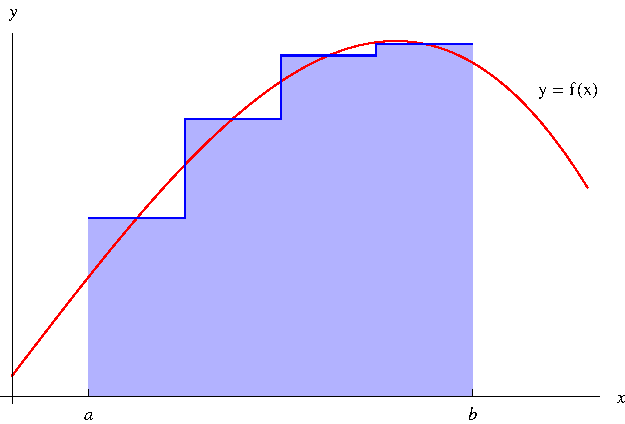
\includegraphics[height=3cm]{area-between-curves/pictures/06-01-4rectangle.pdf}%
%}%
}%
%\only<handout:0| 8>{%
%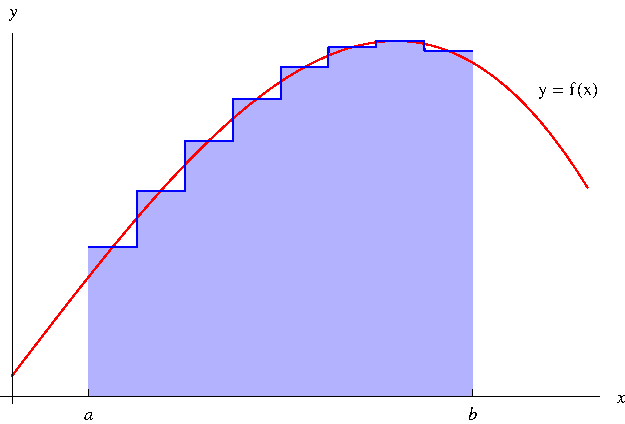
\includegraphics[height=3cm]{area-between-curves/pictures/06-01-8rectangle.pdf}%
%}% 
%\only<handout:0| 9>{%
%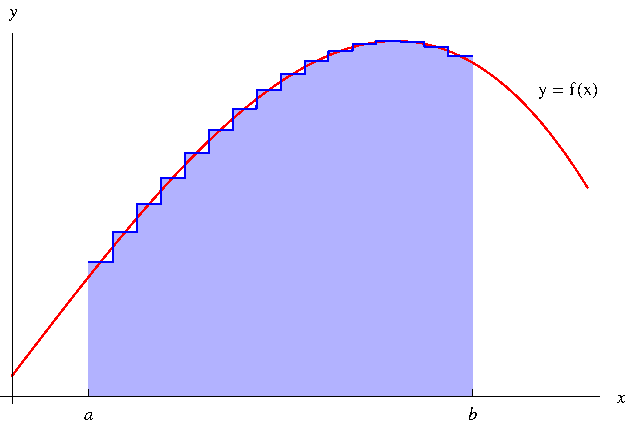
\includegraphics[height=3cm]{area-between-curves/pictures/06-01-16rectangle.pdf}%
%}% 
%\only<handout:0| 10->{%
%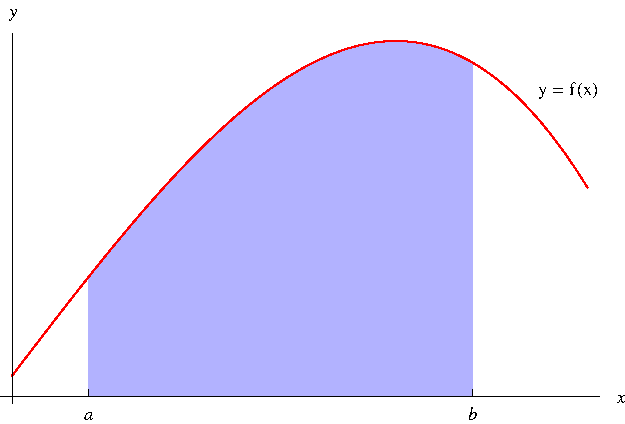
\includegraphics[height=3cm]{area-between-curves/pictures/06-01-singleint.pdf}%
%}
&%
\uncover<18->{ %
\psset{xunit=0.65cm, yunit=0.65cm}
\begin{pspicture}(-0.5, -0.5)(5,5) 
\psframe*[linecolor=white](-0.5,-5)(5,5) 
\tiny 
\psaxes[ticks=none, labels=none]{<->}(0,0)(-0.5,-0.5)(4,3.5)
\psLabels{4}{3.5}
\psXTickWithLabel{0.5}{$a$} 
\psXTickWithLabel{3}{$b$}
\rput[bl](3.1, 3){$y=f(x)$}
\rput[l](3.1, 1.3){$y=g(x)$}

\only<18>{ %
\psline*[linecolor=\psColorAreaUnderGraph, linewidth=0.1pt](0.5, 1.10938)(0.5, 2.01562)(1.125, 2.01562)(1.125, 1.10938)(0.5, 1.10938)
\psline*[linecolor=\psColorAreaUnderGraph, linewidth=0.1pt](1.125, 1.28027)(1.125, 2.0791)(1.75, 2.0791)(1.75, 1.28027)(1.125, 1.28027)
\psline*[linecolor=\psColorAreaUnderGraph, linewidth=0.1pt](1.75, 1.40234)(1.75, 2.19141)(2.375, 2.19141)(2.375, 1.40234)(1.75, 1.40234)
\psline*[linecolor=\psColorAreaUnderGraph, linewidth=0.1pt](2.375, 1.47559)(2.375, 2.35254)(3, 2.35254)(3, 1.47559)(2.375, 1.47559)
\psline[linecolor=blue, linewidth=0.1pt](0.5, 1.10938)(0.5, 2.01562)(1.125, 2.01562)(1.125, 1.10938)(0.5, 1.10938)
\psline[linecolor=blue, linewidth=0.1pt](1.125, 1.28027)(1.125, 2.0791)(1.75, 2.0791)(1.75, 1.28027)(1.125, 1.28027)
\psline[linecolor=blue, linewidth=0.1pt](1.75, 1.40234)(1.75, 2.19141)(2.375, 2.19141)(2.375, 1.40234)(1.75, 1.40234)
\psline[linecolor=blue, linewidth=0.1pt](2.375, 1.47559)(2.375, 2.35254)(3, 2.35254)(3, 1.47559)(2.375, 1.47559)
} %
\only<19>{ %
\psline*[linecolor=\psColorAreaUnderGraph, linewidth=0.1pt](0.5, 1.10938)(0.5, 2.01562)(0.8125, 2.01562)(0.8125, 1.10938)(0.5, 1.10938)
\psline*[linecolor=\psColorAreaUnderGraph, linewidth=0.1pt](0.8125, 1.20093)(0.8125, 2.04126)(1.125, 2.04126)(1.125, 1.20093)(0.8125, 1.20093)
\psline*[linecolor=\psColorAreaUnderGraph, linewidth=0.1pt](1.125, 1.28027)(1.125, 2.0791)(1.4375, 2.0791)(1.4375, 1.28027)(1.125, 1.28027)
\psline*[linecolor=\psColorAreaUnderGraph, linewidth=0.1pt](1.4375, 1.34741)(1.4375, 2.12915)(1.75, 2.12915)(1.75, 1.34741)(1.4375, 1.34741)
\psline*[linecolor=\psColorAreaUnderGraph, linewidth=0.1pt](1.75, 1.40234)(1.75, 2.19141)(2.0625, 2.19141)(2.0625, 1.40234)(1.75, 1.40234)
\psline*[linecolor=\psColorAreaUnderGraph, linewidth=0.1pt](2.0625, 1.44507)(2.0625, 2.26587)(2.375, 2.26587)(2.375, 1.44507)(2.0625, 1.44507)
\psline*[linecolor=\psColorAreaUnderGraph, linewidth=0.1pt](2.375, 1.47559)(2.375, 2.35254)(2.6875, 2.35254)(2.6875, 1.47559)(2.375, 1.47559)
\psline*[linecolor=\psColorAreaUnderGraph, linewidth=0.1pt](2.6875, 1.4939)(2.6875, 2.45142)(3, 2.45142)(3, 1.4939)(2.6875, 1.4939)
\psline[linecolor=blue, linewidth=0.1pt](0.5, 1.10938)(0.5, 2.01562)(0.8125, 2.01562)(0.8125, 1.10938)(0.5, 1.10938)
\psline[linecolor=blue, linewidth=0.1pt](0.8125, 1.20093)(0.8125, 2.04126)(1.125, 2.04126)(1.125, 1.20093)(0.8125, 1.20093)
\psline[linecolor=blue, linewidth=0.1pt](1.125, 1.28027)(1.125, 2.0791)(1.4375, 2.0791)(1.4375, 1.28027)(1.125, 1.28027)
\psline[linecolor=blue, linewidth=0.1pt](1.4375, 1.34741)(1.4375, 2.12915)(1.75, 2.12915)(1.75, 1.34741)(1.4375, 1.34741)
\psline[linecolor=blue, linewidth=0.1pt](1.75, 1.40234)(1.75, 2.19141)(2.0625, 2.19141)(2.0625, 1.40234)(1.75, 1.40234)
\psline[linecolor=blue, linewidth=0.1pt](2.0625, 1.44507)(2.0625, 2.26587)(2.375, 2.26587)(2.375, 1.44507)(2.0625, 1.44507)
\psline[linecolor=blue, linewidth=0.1pt](2.375, 1.47559)(2.375, 2.35254)(2.6875, 2.35254)(2.6875, 1.47559)(2.375, 1.47559)
\psline[linecolor=blue, linewidth=0.1pt](2.6875, 1.4939)(2.6875, 2.45142)(3, 2.45142)(3, 1.4939)(2.6875, 1.4939)
} %
\only<20>{ %
\psline*[linecolor=\psColorAreaUnderGraph, linewidth=0.1pt](0.5, 1.10938)(0.5, 2.01562)(0.65625, 2.01562)(0.65625, 1.10938)(0.5, 1.10938)
\psline*[linecolor=\psColorAreaUnderGraph, linewidth=0.1pt](0.65625, 1.15668)(0.65625, 2.02692)(0.8125, 2.02692)(0.8125, 1.15668)(0.65625, 1.15668)
\psline*[linecolor=\psColorAreaUnderGraph, linewidth=0.1pt](0.8125, 1.20093)(0.8125, 2.04126)(0.96875, 2.04126)(0.96875, 1.20093)(0.8125, 1.20093)
\psline*[linecolor=\psColorAreaUnderGraph, linewidth=0.1pt](0.96875, 1.24213)(0.96875, 2.05865)(1.125, 2.05865)(1.125, 1.24213)(0.96875, 1.24213)
\psline*[linecolor=\psColorAreaUnderGraph, linewidth=0.1pt](1.125, 1.28027)(1.125, 2.0791)(1.28125, 2.0791)(1.28125, 1.28027)(1.125, 1.28027)
\psline*[linecolor=\psColorAreaUnderGraph, linewidth=0.1pt](1.28125, 1.31537)(1.28125, 2.1026)(1.4375, 2.1026)(1.4375, 1.31537)(1.28125, 1.31537)
\psline*[linecolor=\psColorAreaUnderGraph, linewidth=0.1pt](1.4375, 1.34741)(1.4375, 2.12915)(1.59375, 2.12915)(1.59375, 1.34741)(1.4375, 1.34741)
\psline*[linecolor=\psColorAreaUnderGraph, linewidth=0.1pt](1.59375, 1.3764)(1.59375, 2.15875)(1.75, 2.15875)(1.75, 1.3764)(1.59375, 1.3764)
\psline*[linecolor=\psColorAreaUnderGraph, linewidth=0.1pt](1.75, 1.40234)(1.75, 2.19141)(1.90625, 2.19141)(1.90625, 1.40234)(1.75, 1.40234)
\psline*[linecolor=\psColorAreaUnderGraph, linewidth=0.1pt](1.90625, 1.42523)(1.90625, 2.22711)(2.0625, 2.22711)(2.0625, 1.42523)(1.90625, 1.42523)
\psline*[linecolor=\psColorAreaUnderGraph, linewidth=0.1pt](2.0625, 1.44507)(2.0625, 2.26587)(2.21875, 2.26587)(2.21875, 1.44507)(2.0625, 1.44507)
\psline*[linecolor=\psColorAreaUnderGraph, linewidth=0.1pt](2.21875, 1.46185)(2.21875, 2.30768)(2.375, 2.30768)(2.375, 1.46185)(2.21875, 1.46185)
\psline*[linecolor=\psColorAreaUnderGraph, linewidth=0.1pt](2.375, 1.47559)(2.375, 2.35254)(2.53125, 2.35254)(2.53125, 1.47559)(2.375, 1.47559)
\psline*[linecolor=\psColorAreaUnderGraph, linewidth=0.1pt](2.53125, 1.48627)(2.53125, 2.40045)(2.6875, 2.40045)(2.6875, 1.48627)(2.53125, 1.48627)
\psline*[linecolor=\psColorAreaUnderGraph, linewidth=0.1pt](2.6875, 1.4939)(2.6875, 2.45142)(2.84375, 2.45142)(2.84375, 1.4939)(2.6875, 1.4939)
\psline*[linecolor=\psColorAreaUnderGraph, linewidth=0.1pt](2.84375, 1.49847)(2.84375, 2.50543)(3, 2.50543)(3, 1.49847)(2.84375, 1.49847)
\psline[linecolor=blue, linewidth=0.1pt](0.5, 1.10938)(0.5, 2.01562)(0.65625, 2.01562)(0.65625, 1.10938)(0.5, 1.10938)
\psline[linecolor=blue, linewidth=0.1pt](0.65625, 1.15668)(0.65625, 2.02692)(0.8125, 2.02692)(0.8125, 1.15668)(0.65625, 1.15668)
\psline[linecolor=blue, linewidth=0.1pt](0.8125, 1.20093)(0.8125, 2.04126)(0.96875, 2.04126)(0.96875, 1.20093)(0.8125, 1.20093)
\psline[linecolor=blue, linewidth=0.1pt](0.96875, 1.24213)(0.96875, 2.05865)(1.125, 2.05865)(1.125, 1.24213)(0.96875, 1.24213)
\psline[linecolor=blue, linewidth=0.1pt](1.125, 1.28027)(1.125, 2.0791)(1.28125, 2.0791)(1.28125, 1.28027)(1.125, 1.28027)
\psline[linecolor=blue, linewidth=0.1pt](1.28125, 1.31537)(1.28125, 2.1026)(1.4375, 2.1026)(1.4375, 1.31537)(1.28125, 1.31537)
\psline[linecolor=blue, linewidth=0.1pt](1.4375, 1.34741)(1.4375, 2.12915)(1.59375, 2.12915)(1.59375, 1.34741)(1.4375, 1.34741)
\psline[linecolor=blue, linewidth=0.1pt](1.59375, 1.3764)(1.59375, 2.15875)(1.75, 2.15875)(1.75, 1.3764)(1.59375, 1.3764)
\psline[linecolor=blue, linewidth=0.1pt](1.75, 1.40234)(1.75, 2.19141)(1.90625, 2.19141)(1.90625, 1.40234)(1.75, 1.40234)
\psline[linecolor=blue, linewidth=0.1pt](1.90625, 1.42523)(1.90625, 2.22711)(2.0625, 2.22711)(2.0625, 1.42523)(1.90625, 1.42523)
\psline[linecolor=blue, linewidth=0.1pt](2.0625, 1.44507)(2.0625, 2.26587)(2.21875, 2.26587)(2.21875, 1.44507)(2.0625, 1.44507)
\psline[linecolor=blue, linewidth=0.1pt](2.21875, 1.46185)(2.21875, 2.30768)(2.375, 2.30768)(2.375, 1.46185)(2.21875, 1.46185)
\psline[linecolor=blue, linewidth=0.1pt](2.375, 1.47559)(2.375, 2.35254)(2.53125, 2.35254)(2.53125, 1.47559)(2.375, 1.47559)
\psline[linecolor=blue, linewidth=0.1pt](2.53125, 1.48627)(2.53125, 2.40045)(2.6875, 2.40045)(2.6875, 1.48627)(2.53125, 1.48627)
\psline[linecolor=blue, linewidth=0.1pt](2.6875, 1.4939)(2.6875, 2.45142)(2.84375, 2.45142)(2.84375, 1.4939)(2.6875, 1.4939)
\psline[linecolor=blue, linewidth=0.1pt](2.84375, 1.49847)(2.84375, 2.50543)(3, 2.50543)(3, 1.49847)(2.84375, 1.49847)
} %
\only<21->{ %
\pscustom*[linecolor=\psColorAreaUnderGraph]{
%Function formula: 3/2- ((-3/4+1/4 (x))^{2}) 
\psplot[plotpoints=1000]{0.5}{3}{x 0.25 mul -0.75 add 2 exp -1 mul 1.5 add }
%Function formula: (1/4 (x))^{2}+2 
\psplot[plotpoints=1000]{3}{0.5}{2 x 0.25 mul 2 exp add }
} %
} %
%Function formula: 3/2- ((-3/4+1/4 (x))^{2}) 
\psplot[linecolor=\psColorGraph, plotpoints=1000]{0}{4}{x 0.25 mul -0.75 add 2 exp -1 mul 1.5 add }
%Function formula: (1/4 (x))^{2}+2 
\psplot[linecolor=\psColorGraph, plotpoints=1000]{0}{4}{2 x 0.25 mul 2 exp add }
\end{pspicture} 
} %
%\ \only<-18>{%
%\uncover<18->{%
%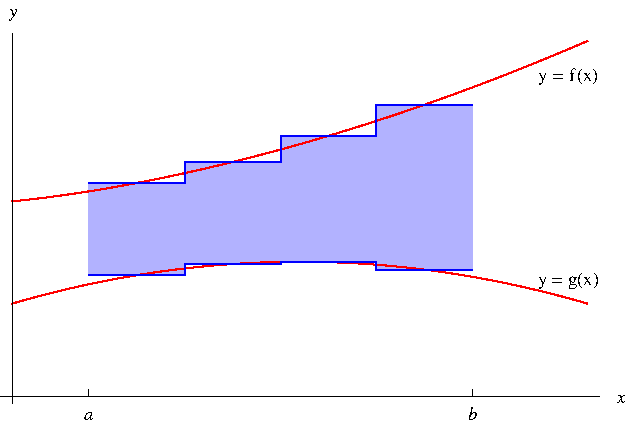
\includegraphics[height=3cm]{area-between-curves/pictures/06-01-4rectanglediff.pdf}%
%}%
%}%
%\only<handout:0| 19>{%
%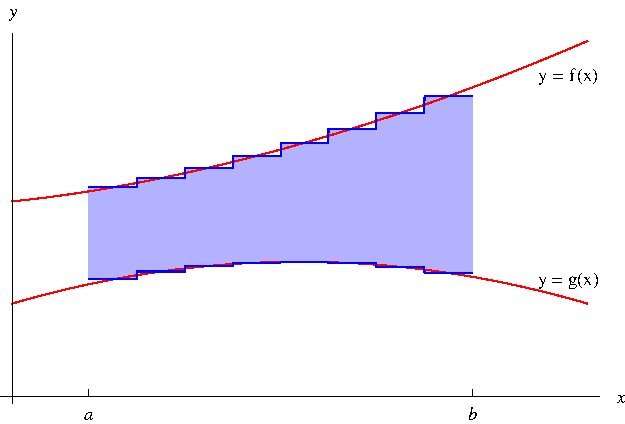
\includegraphics[height=3cm]{area-between-curves/pictures/06-01-8rectanglediff.pdf}%
%}%  
%\only<handout:0| 20>{%
%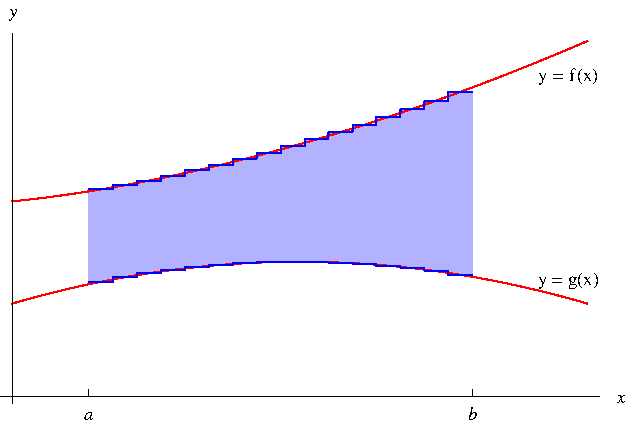
\includegraphics[height=3cm]{area-between-curves/pictures/06-01-16rectanglediff.pdf}%
%}%  
%\only<handout:0| 21>{%
%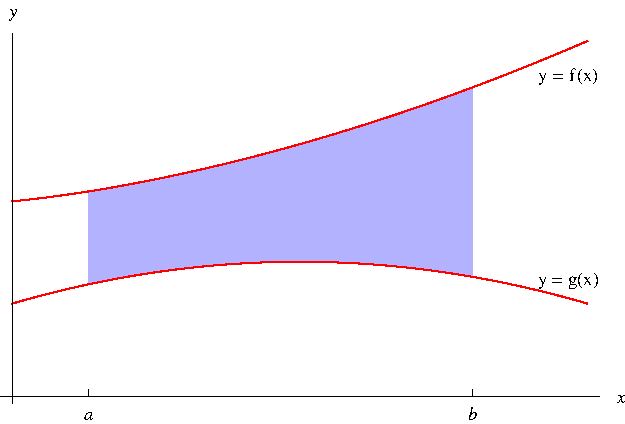
\includegraphics[height=3cm]{area-between-curves/pictures/06-01-doubleint.pdf}%
%}
\\
\uncover<7->{
\# rectangles $ = \alert<handout:0| 10>{n} \only<handout:0| -9>{=}\only<10->{\alert<handout:0| 10>{\rightarrow}} $ \only<handout:0| -7>{4}\only<handout:0| 8>{\alert<handout:0| 8>{8}}\only<handout:0| 9>{\alert<handout:0| 9>{16}}\only<10->{\alert<handout:0| 10>{$\infty$}}
} & 
\uncover<18->{
\# rectangles $ = n \only<handout:0| -20>{=}\only<21->{\rightarrow} $ \only<handout:0| -18>{4}\only<handout:0| 19>{8}\only<handout:0| 20>{16}\only<21->{$\infty$}
} \\
\only<handout:0| -9,12->{\invisible<1->{$\underset{n\rightarrow \infty}{\lim}$}}%
\uncover<7->{
A  =  \only<handout:0| 10-11>{\alert<handout:0| 10-11>{$\underset{n\rightarrow \infty}{\lim}$}}\only<handout:0| -11>{\alert<handout:0| 11>{$ \sum_{i = 1}^{\only<handout:0| -7>{4}\only<handout:0| 8>{\alert<handout:0| 8>{8}}\only<handout:0| 9>{\alert<handout:0| 9>{16}}\only<handout:0| 10->{\alert<handout:0| 10>{n}}} f(x_i)\Delta x$}}
\only<12->{\alert<handout:0| 12>{$ \int_a^b f(x)\diff x$}}
}% 
\only<-11>{\invisible<1->{$\int_a^b$}}%
& 
\uncover<18->{
A  =  \only<handout:0| -20>{$ \sum_{i = 1}^{\only<handout:0| -18>{4}\only<handout:0| 19>{8}\only<handout:0| 20>{16}} (f(x_i)- g(x_i))\Delta x$}
\only<21->{$ \int_a^b [f(x) - g(x)]\diff x$}
} \\ 
\hline
\end{tabular}
\end{frame}


\begin{frame}
\begin{definition}[The Area Between Two Curves]
The area between two curves $y = f(x)$ and $y = g(x)$ bounded by the endpoints $x = a$ and $x = b$ is
\[ \int_a^b |f(x) - g(x)|\diff x . \]

Note that we use the absolute value, because in general we don't know which curve is above the other.
\end{definition}
\end{frame}
% end module area-between-curves-def
